\documentclass[12pt]{standalone}

\usepackage{tikz}
\usepackage{ctex}

\tikzset{graph node/.style={circle,draw}}
\tikzset{weight/.style={node font=\footnotesize}}

\begin{document}
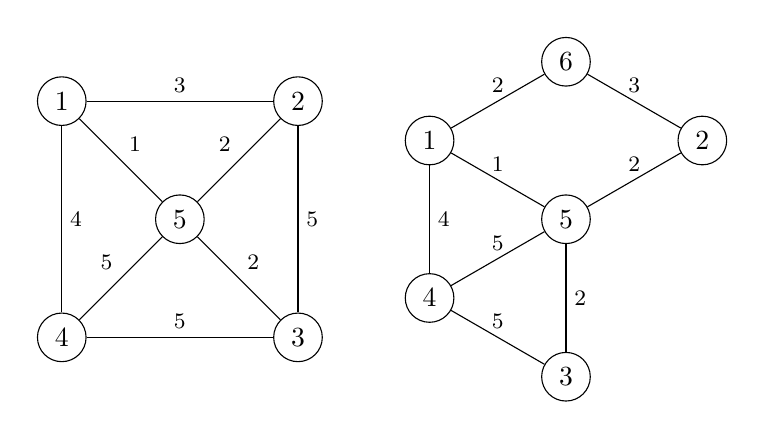
\begin{tikzpicture}[x=15mm,y=15mm]

    \matrix[column sep=1cm] {
        \node[graph node] (1) at (-1,1) {1};
        \node[graph node] (2) at (1,1) {2};
        \node[graph node] (3) at (1,-1) {3};
        \node[graph node] (4) at (-1,-1) {4};
        \node[graph node] (5) at (0,0) {5};
        
        \draw (1) -- node[weight,above] {3} (2);
        \draw (1) -- node[weight,above right] {1} (5);
        \draw (1) -- node[weight,right] {4} (4);
        \draw (2) -- node[weight,right] {5} (3);
        \draw (2) -- node[weight,above left] {2} (5);
        \draw (4) -- node[weight,above] {5} (3);
        \draw (4) -- node[weight,above left] {5} (5);
        \draw (5) -- node[weight,above right] {2} (3);
        &
        \begin{scope}[x=1cm,y=1cm]
            \node[graph node] (1) at (0,1) {1};
            \node[graph node] (2) at (3.46410,1) {2};
            \node[graph node] (3) at (1.73205,-2) {3};
            \node[graph node] (4) at (0,-1) {4};
            \node[graph node] (5) at (1.73205,0) {5};
            \node[graph node] (6) at (1.73205,2) {6};

            \draw (1) -- node[weight,right] {4} (4);
            \draw (1) -- node[weight,above] {1} (5);
            \draw (1) -- node[weight,above] {2} (6);
            \draw (4) -- node[weight,above] {5} (3);
            \draw (4) -- node[weight,above] {5} (5);
            \draw (5) -- node[weight,right] {2} (3);
            \draw (5) -- node[weight,above] {2} (2);
            \draw (6) -- node[weight,above] {3} (2);
        \end{scope}
        \\
    };

\end{tikzpicture}
\end{document}
